\documentclass[12pt]{article}

\usepackage{url}
\usepackage[backend=bibtex,sorting=none]{biblatex}
\usepackage{dirtytalk}
\usepackage{amsmath,amssymb,mathtools,bm,etoolbox}
\usepackage{listings}
\usepackage{graphicx}
\usepackage{float}

\graphicspath{ {images/} }

\lstset{frame=tb,
  language=Erlang,
  aboveskip=3mm,
  belowskip=3mm,
  showstringspaces=false,
  columns=flexible,
  basicstyle={\small\ttfamily},
  numbers=none,
  numberstyle=\tiny
  breaklines=true,
  breakatwhitespace=true,
  tabsize=2,
  literate={\ \ }{{\ }}1}

\newlength\tindent
\setlength{\tindent}{\parindent}
\setlength{\parindent}{0pt}
\renewcommand{\indent}{\hspace*{\tindent}}

\bibliography{hll}

\begin{document}

\title{Hyperloglog Datatypes in Riak}
\author{Zeeshan Lakhani}

\maketitle

\section{Getting Started}

Hyperloglog (HLL) was conceived of by
Flajolet et.al.\cite{Flatjolet:2007:Online} in 2007 as an improvement and
extension on the Loglog\cite{Durand:2003:Online} algorithm to tackle the
\textbf{Count-distinct problem}\cite{Count-distinct:Online}, or finding the
number of distinct elements in a large file and, later, a data stream.
Or, as more properly stated in the quintessential 2007 paper:\newline

\say{The purpose of this note is to present and analyse an efficient algorithm
for estimating the number of distinct elements, known as the cardinality, of
large data ensembles, which are referred to here as multisets and are usually
massive streams (read-once sequences). This problem has received a great deal of
attention over the past two decades, finding an ever growing number of
applications in networking and traffic monitoring, such as the detection of worm
propagation, of network attacks (e.g., by Denial of Service), and of link-based
spam on the web.}

\subsection{Why HyperLogLog?}

So, what's a good use case for HLLs? One example would be to determine the
number of distinct search queries on \textit{google.com} over a time
period\cite{Heule:2013:Online}.

\indent The goal of HLL is to estimate unique elements in large sets (large being beyond
$10^{9}$) and streams while also keeping memory low(er). Normally, calculating
the exact cardinality of a set requires an amount of memory proportional to the
cardinality when counting these unique items. With HLLs, the trade off is less
memory in exchange for approximated cardinality. Yo performance.\newline

As per \cite{Heule:2013:Online}, the key requirements for cardinality an
estimation algorithm are

\begin{enumerate}
\item \textbf{Accuracy}: For a fixed amount of memory, the algorithm should
  provide as accurate an estimate as possible. Especially for small
  cardinalities, the results should be near exact.
\item \textbf{Memory efficiency}: The algorithm should use the available memory
  efficiently and adapt its memory usage to the cardinality. That is, the
  algorithm should use less than the user-specified maximum amount of memory if
  the cardinality to be estimated is very small.
\item \textbf{Estimate large cardinalities}: Multisets with cardinalities well
  beyond 1 billion occur on a daily basis, and it is important that such large
  cardinalities can be estimated with reasonable accuracy.
\item \textbf{Practicality}: The algorithm should be implementable and
  maintainable.
\end{enumerate}

There are two generalized categories of cardinality observables
\cite{Flatjolet:2007:Online}:

\begin{enumerate}
\item \textbf{Bit-pattern observables}: these are based on certain patterns of
  bits occurring at the beginning of the (binary) $S$-values. For instance,
  observing in the stream $S$ at the beginning of a string a bitpattern
  $0^{p-1}1$ is more or less a likely indication that the cardinality $n$
  of $S$ is at least $2^{p}$. HLL is an example of this category.

\item \textbf{Order statistics observables}: these are based on order statistics,
  like the smallest (real) values, that appear in $S$. For instance,
  if $X = min(S)$, we may legitimately hope that $n$ is roughly of the order of
  $1/X$, since, as regards expectations, one has $\mathbb{E}(X) = 1/(n + 1)$.
\end{enumerate}

\section{The HyperLogLog Algorithm}

\indent The key components of the algorithm are

\begin{enumerate}
\item \textit{randomization achieved by a hash function}, $h$, which is applied
  to every element which is counted bits.
\item As a hashed valued comes in, the first $p$, \texttt{precision}
  \texttt{(4..16)} bits are used to determine which register (substream) which
  we'll use to store the maximum number of leading zeros in the rest of the
  hash. The \textit{bit-pattern observables} in the HLL approach would be this
  maximum, aka the longest run of zeros in the hash values (after the initial
  $p$ bits). $m = 2^p$ is the maximum number of hash values maintained.
\item \textit{stochastic averaging} across the
  registers/substreams\textemdash divided $m$ substreams of $S_i$
  ($S$ meaning data elements), to reduce the large variability of each single
  measurement.
\item To reduce dramatic outliers, a \textit{harmonic mean} is used instead of
  a arithmetic mean across the estimates, which tends strongly tward the least
  elements of the list\cite{Harmonic-mean:Online}.
\end{enumerate}

Here's a visualization of the basic idea\cite{Kiip:Online}:

\begin{figure}[H]
\centering
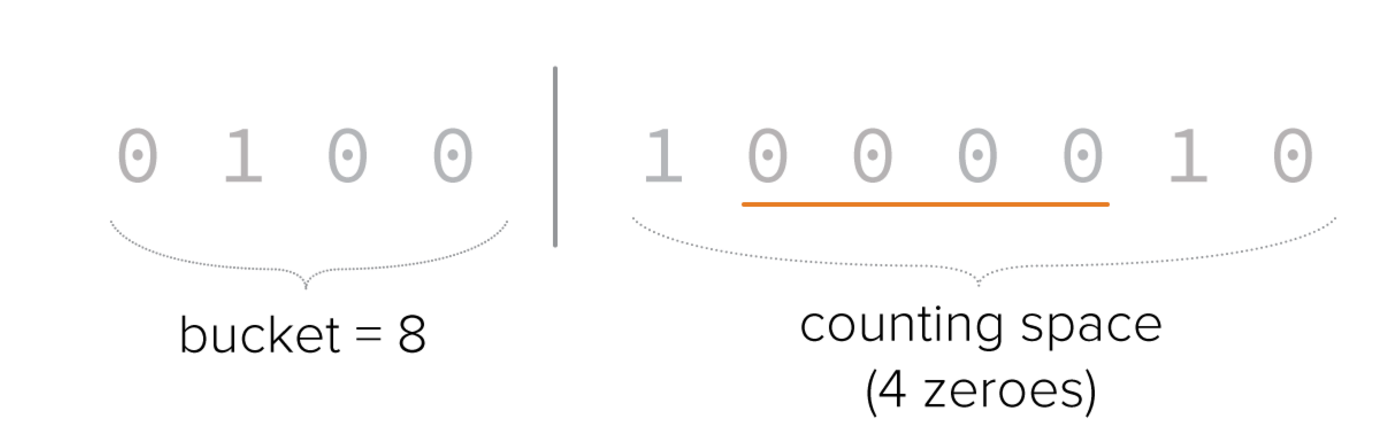
\includegraphics[width=8.1cm, height=4cm]{bucket-run}
\caption{$p=4$; The bucket/register for the hashed value of $0100$ is $8$.}
\label{figurebucketrun}
\end{figure}

\begin{figure}[H]
\centering
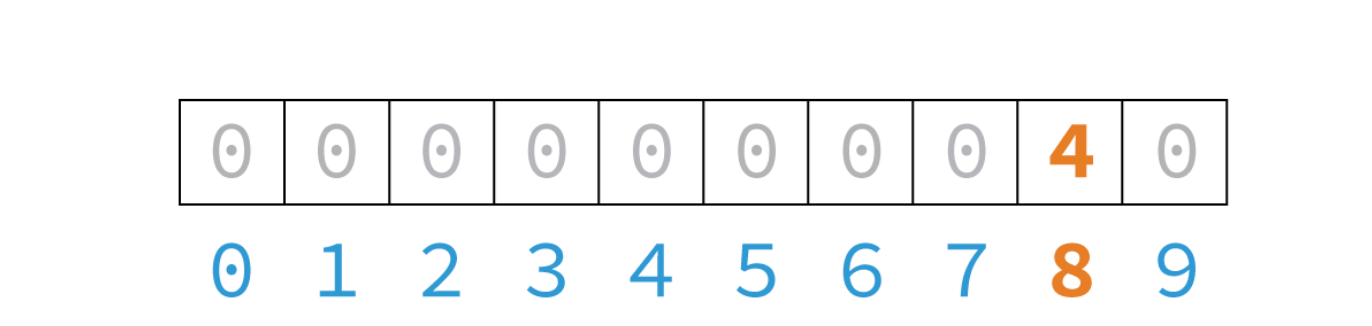
\includegraphics[width=8.2cm, height=3cm]{register-store}
\caption{Storing 4 as the max number of leading zeros.}
\label{figurestoreregister}
\end{figure}

\begin{figure}[H]
\centering
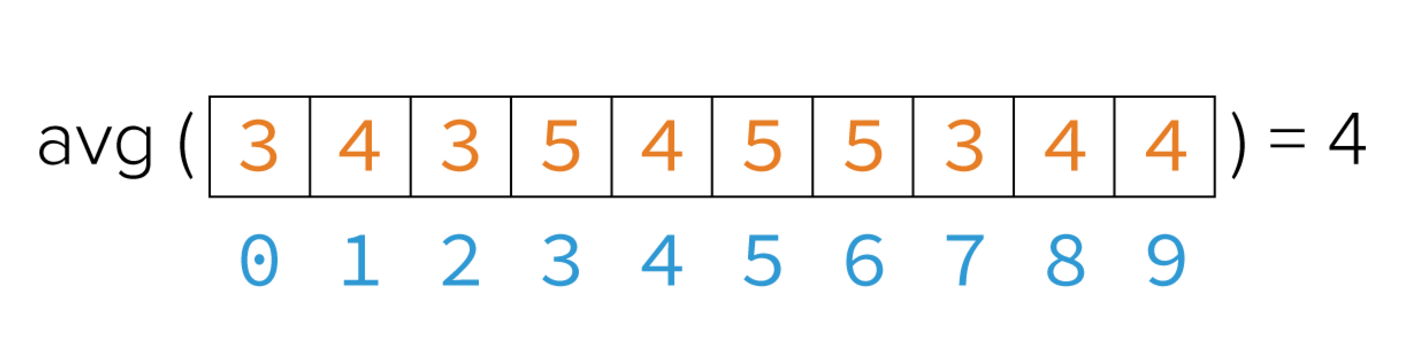
\includegraphics[width=8.0cm, height=3cm]{sto-avg}
\caption{To reduce the large variability of single measurements, a stochastic
  average is calculated across the registers. \textbf{This is a simple example}.
  A normalized bias corrected harmonic mean of the estimations is actually used
  for the final estimate.}
\label{figurestoaverage}
\end{figure}

The simplified formula that actually defines the HLL distinct-value (DV)
estimator\cite{Neustar:Online} is

$$DV_{HLL} = constant * m^{2} * \Bigg(\sum_{j=1}^{m} 2^{-R_{j}}\Bigg)^{-1}$$

$R_j$ is the longest run of zeroes in the $j^{th}$ bucket. The relative error
is $1.04/\sqrt{m}$ ($m$ - number of counters). More information about the
original algorithm and it's additional modifications can be found in
\cite{Flatjolet:2007:Online}.

\subsection{HyperLogLog++}\label{hll++}

As per \cite{Heule:2013:Online}, going into production with requirements of
estimating multisets of cardinalities beyond 1 billion, there needed to be
some changes to the known HLL algorithm, hence \textit{HyperLogLog++}.\newline

The main changes we'll take away for this exercise are

\begin{enumerate}
\item Use a 64-bit hash function instead of the
  original's\cite{Flatjolet:2007:Online} 32-bit hash function with special range
  correction. Therefore, hash collisions only become a problem if we reach a
  cardinality of $2^{64}$, which is fine for many real-world data sets.
\item HyperLogLog++ introduces a bias-correction which corrects for bias
  using empirically determined data for cardinalities $< 5m$.
\end{enumerate}

\section{HLL Datatypes in Riak}

\subsection{Hyper Library}

Our HyperLogLogs (HLLs) are driven by GameAnalytics' Erlang HyperLogLog
implementation\cite{Hyper:Online} under the hood, which includes the bias
correction from \cite{Heule:2013:Online} (mentioned in \ref{hll++}).

\indent Currently, we are using the \textit{hyper\_binary} option as a backend,
which has \say{fixed memory usage $(6 bits * 2^{P})$, fastest on insert, union,
  cardinality and serialization. Best default choice.} 6 instead of 5 bits is
mentioned due to the increased-bit hash function.

\indent The library gives us the ability to perform unions
(\textit{looks like a merge}), be prescribed a precision, reduce precision,
union varying-precisioned HLLs (based on a \textit{union} toward the reduced
HLL), and compact the data structure's buffer before the registers are
needed/calculated from.\newline

Here's an example of what an insert and card-check looks like:

\begin{lstlisting}
H = hyper:insert(<<"foo">>, hyper:insert(<<"qu">>, hyper:new(4))).
{hyper,4,
    {hyper_binary,{dense,<<0,0,0,0,0,0,0,0,0,0,0,2>>,[{0,1}],1,16}}}

hyper:card(H).
2.136502281992361
\end{lstlisting}

\subsection{Brief In-Riak Example}

Ok. Here's an example workflow with the Riak erlang-(pb)-client:

\begin{lstlisting}
CMod = riakc_pb_socket,
Key = <<"Holy Diver">>,
Bucket = {<<"hll_bucket">>, <<"testbucket1">>},

S0 = riakc_hll:new(),

Item = <<"Jokes">>,
ok = CMod:update_type(
                     Pid, Bucket, Key, riakc_hll:to_op(
                     riakc_hll:add_element(Item, S0))
                    ).

{ok, S1} = CMod:fetch_type(Pid, Bucket, Key),
Items = [<<"are">>, <<"better">>, <<"explained">>],
ok = CMod:update_type(
                     Pid, Bucket, Key,
                     riakc_hll:to_op(riakc_hll:add_elements(Items, S1))
                    ).

{ok, S2} = CMod:fetch_type(Pid, Bucket, Key),
riakc_hll:value(S2) =:= 4.

%% Add a redundant element

ok = CMod:update_type(
                     Pid, Bucket, Key, riakc_hll:to_op(
                     riakc_hll:add_element(Item, S2))
                    ).

{ok, S3} = CMod:fetch_type(Pid, Bucket, Key),
riakc_hll:value(S3) =:= 4.
\end{lstlisting}

\subsection{Testing within an Error Bound}

\begin{lstlisting}
%% @doc Standard Error is sigma ≈ 1.04/srqt(m), where m is the
%% # of registers. Deviations are related to margin of error away
%% from the actual cardinality in of percentils.
%% sigma = 65%, 2σ=95%, 3σ=99%
margin_of_error(P, Deviations) ->
    M = trunc(math:pow(2, P)),
    Sigma = 1.04 / math:sqrt(M),
    Sigma*Deviations.

%% @doc Check if Estimated Card from HllSet is within an acceptable
%% margin of error determined by m-registers and 3 deviations of
%% the standard error. Use a window of +1 to account for rounding
%% and extremely small cardinalities.
within_error_check(Card, HllSet, HllVal) ->
    case Card > 0 of
        true ->
            Precision = riak_dt_hll:precision(HllSet),
            MarginOfError = margin_of_error(Precision, 3),
            RelativeError = (abs(Card-HllVal)/Card),
            %% Is the relative error within the margin of error times
            %% the estimation *(andalso)* is the value difference less than
            %% the actual cardinality times the margin of error
            BoundCheck1 = RelativeError =< (MarginOfError * HllVal)+1,
            BoundCheck2 = abs(HllVal-Card) =< (Card*MarginOfError)+1,
            BoundCheck1 andalso BoundCheck2;
        _ -> trunc(HllVal) == Card
    end.
\end{lstlisting}

\section{So?}

So, HLL's are a super useful way to count distinct elements in a set, stream,
multiset while also keeping memory and data structure byte-size down. Win!

\printbibliography

\end{document}
